\scanpage{73}
$I'$, $I''$, les $I'_\alpha$ sont des parties de $I$ satisfaisant (7) (des \uline{cribles} de $I$)

Si dans A) on prend $X'=X$, il est plus commode de travailler avec la stratification de $X'$ définie par les $X_i$ où $i\in I'$ --- Il est clair que les \unsure{conditions} (11) relatives à $X'=X_{I'}$ sont satisfaites. Les ``parties cribles'' de $X'$ pour cette stratification, ou pour celle induite au sens général des espaces au dessus de $X$, sont les $\unsure{=^{\mathrm s}|\overline{\mathrm m}^{\mathrm s}}$ --- ce sont \inserted{donc} les traces \deleted{\unsure{inverses}} \inserted{sur} $X'=X_{I'}$ des parties-cribles de l'espace stratifié $X$.

Ici, les espaces élémentaires pour la stratification de type $I'$ de \deleted{\unsure{X}} $X'=X_{\unsure{I'|J'}}$, sont les espaces
\[
(12)\quad \figure{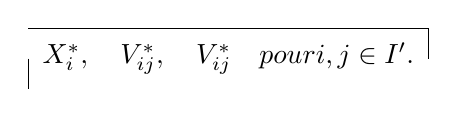
\begin{tikzpicture}
\node[inner sep=5pt] (f) {$X_i^*,\quad V_{ij}^*,\quad V_{ij}^{\deleted{\unsure{*}}}\quad\text{pour }i,j\in I'.$};
\draw (f.north west)--(f.north east)--(f.east);
\draw (f.west)--(f.south west);
\end{tikzpicture}}
\]

\deleted{Combinant les deux opérations, \unsure{on a} p.ex. une stratification pour \unsure{tt} ouvert $U'$ d'un $X'=X_{I'}$, avec les espaces élémentaires associés, qui sont donc les
\[
(13)\quad U'\cap X_i^*,\quad U'\cap V_{ij}^*,\quad U'\cap V_{ij}\qquad(i,j\in I')
\]}

\mspage{72}
